\documentclass[11pt,border=5pt]{standalone}
\usepackage{fontspec}
\setmainfont{cmunrm.otf}[BoldFont=cmunbx.otf,ItalicFont=cmunti.otf,BoldItalicFont=cmunbi.otf]
\usepackage{amsmath}
\usepackage{unicode-math}
\setmathfont{NewCMMath-Regular.otf}
\usepackage{tikz}
\usetikzlibrary{arrows.meta,patterns,angles,quotes}
\begin{document}
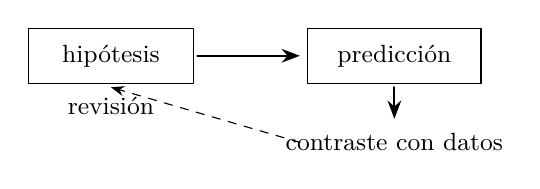
\begin{tikzpicture}[>=Stealth,font=\small,line cap=round,line join=round]
\draw[fill=white] (-3.05,-0.35) rectangle (-0.95,0.35);
\node at (-2,0) {hipótesis};
\draw[->,thick] (-0.9,0) -- (0.4,0);
\draw[fill=white] (0.5,-0.35) rectangle (2.7,0.35);
\node at (1.6,0) {predicción};
\node at (1.6,-1.1) {contraste con datos};
\draw[->,thick] (1.6,-0.4) -- (1.6,-0.8);
\draw[->,thin,dashed] (0.4,-1.1) -- (-2,-0.4) node[below] {revisión};

\end{tikzpicture}
\end{document}
